\documentclass[a4paper,12pt]{article}
\usepackage[bahasa]{babel}
\usepackage{graphicx}
\usepackage{multirow}
\usepackage{enumitem}
\usepackage{listings}
\usepackage{adjustbox}
\graphicspath{ {./img/} }
\begin{document}
\title{Laporan Praktikum Statistika Pertemuan 10}
%\author{Aldzikri Dwijayanto Prathama \\ {\small 195410189}}
\author{Aldzikri Dwijayanto Prathama 
	\\195410189}
\makeatletter
\begin{titlepage}
	\begin{center}
		{\huge \bfseries \@title }\\[14ex]
		
\includegraphics[scale=.8]{logo}\\[4ex]
		{\large \@author}\\[20ex]
		{\large \bfseries {SEKOLAH TINGGI MANAJEMEN INFORMATIKA DAN KOMPUTER
				AKAKOM YOGYAKARTA}}
	\end{center}


%{\large \@date} 
\end{titlepage}
\makeatother
%\maketitle
\newpage
\tableofcontents
\newpage
\section{Pembahasan}
Probabilitas adalah kemungkinan yang dapat terjadi dalam suatu peristiwa tertentu. Definisi probabilitas dapat dilihat dari tiga macam pendekatan, yaitu pendekatan klasik, pendekatan frekuensi relatif dan pendekatan subjektif.

\subsection{Praktik}
\subsubsection{Praktik 1}
Pada praktik 1 digunakan pendekatan klasik, menurut pendekatan klasik pada suatu peristiwa random dapat terjadi dalam n cara yang masing-masing memiliki kemungkinan yang sama, dan apabila sejumlah n(B) digunakan untuk cara memberikan hasil B.
\begin{center}
	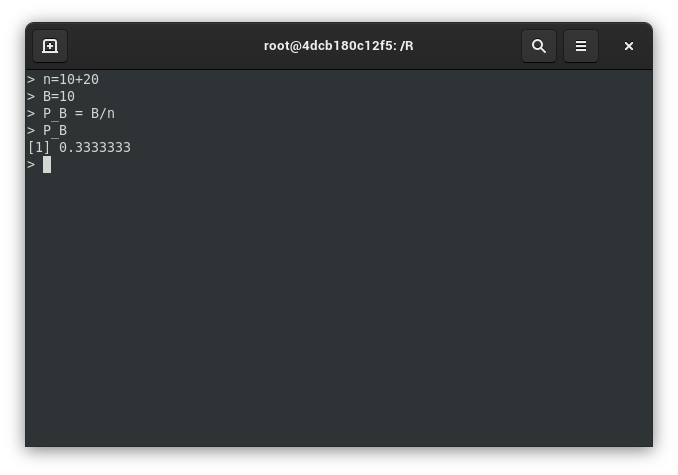
\includegraphics[scale=.5]{prak1}
\end{center}
Pada R Console kita ketikkan\\
\texttt{n=10+20}\\
artinya kita memberi nilai n dengan 10 butir telur bebek ditambah dengan 20 butir telur ayam yaitu 30 butir telur, kemudian klik enter. Selanjutnya kita ketikkan \\
\texttt{B=10}\\
artinya B adalah 10 butir telur. Kemudian kita beri rumus\\ 
\texttt{P\_B = B/n }, kemudian kita panggil lagi P\_B. Maka peluang terambil telur bebek adalah 0,33333.

\subsubsection{Praktik 2}
Praktik 2 adalah menentukan peluang berapa warna merah atau hijau yang terambil dari kotak jika kelereng diambil secara acak dengan mata  tertutup. Diketahui A = mengambil warna merah, B = mengambil warna kuning, C = mengambil warna hijau, n(A) = 10, n(B) = 18, n(C) = 22, dan n = n(A) + n(B) + n(C) = 10+18+22.
\begin{center}
	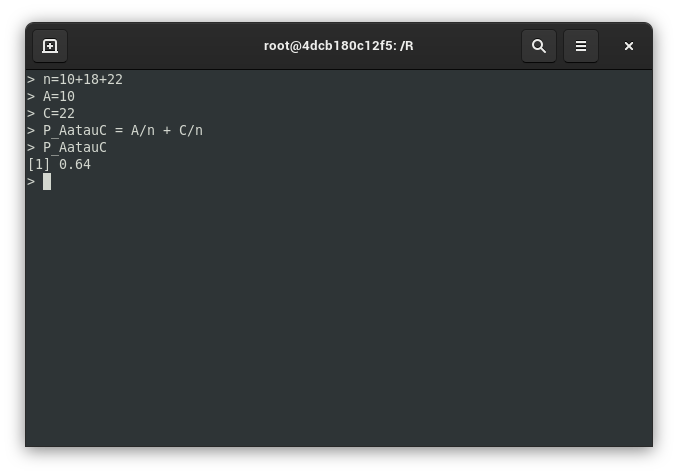
\includegraphics[scale=.5]{prak2}
\end{center} 
Peristiwa tersebut termasuk peristiwa saling lepas. Dua peristiwa atau lebih disebut peristiwa saling lepas apabila kedua atau lebih peristiwa tersebut tidak bisa terjadi pada saat bersamaan. Untuk dua peristiwa A dan peristiwa B yang saling lepas, maka probabilitas terjadinya peristiwa tersebut adalah sebagai berikut:
\[ P(A \cup B) = P(A)+P(B) \]

Jadi pada R Console dibawah kita ketikkan\\ 
\texttt{n=10+18+22}\\
yang artinya kita memberi nilai n dengan 10 kelereng merah ditambah 18 kelereng hijau ditambah 22 kelereng kuning yaitu 50 butir kelereng. Kemudian kita ketikkan\\ 
\texttt{A=10}\\ 
yang artinya A adalah 10 kelereng merah, kemudian kita ketikkan lagi\\ 
\texttt{C=22}\\ 
yang artinya C adalah 22 kelereng kuning, setelah itu kita ketikkan\\  \texttt{P\_AatauC = A/n + C/n}\\ 
Hasil akhir yang didapatkan adalah Peluang terambilnya kelereng warna merah atau kuning adalah 0,64.
 
\subsubsection{Praktik 3}
Praktik 3 adalah menentukan peluang yang terpilih siswa yang menyukai matematika atau bahasa Inggris, dari 45 siswa pada suatu kelas, diketahui 28 siswa senang matematika, 22 siswa bahasa inggris, dan 10 siswa suka kedua-duanya. Jika seorang siswa dipilih secara acak
\begin{center}
	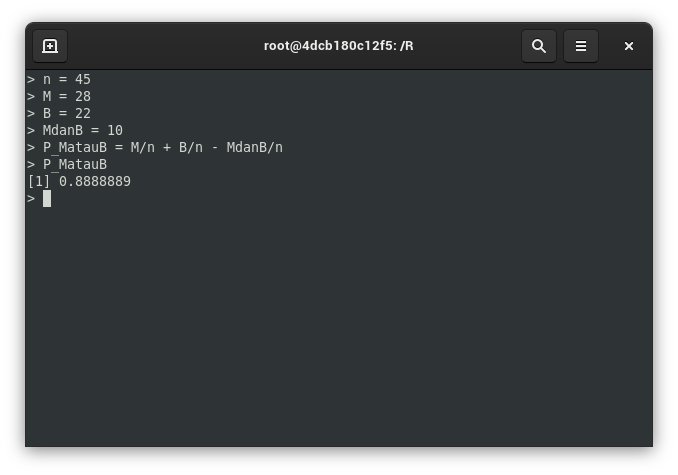
\includegraphics[scale=.5]{prak3}
\end{center}
Peristiwa tersebut termasuk peristiwa tidak saling bebas, karena terjadinya peristiwa yang satu mempengaruhi atau dipengaruhi terjadinya peristiwa yang lainnya. Untuk dua peristiwa A dan B yang tidak saling bebas, probabilitas terjadinya peristiwa tersebut adalah sebagai berikut:
\[ P(A \cap B) = P(A) P(B|A) \]
Diketahui M = suka matematika, B = suka Bahasa inggris, n = 45 artinya banyaknya data dari praktik ini adalah 45, kemudia n(M) = 28 artinya banyaknya yang suka matematika, n(B) = 22 adalah banyaknya yang suka Bahasa inggris, dan n(M Ç B) = 10 artinya banyaknya yang suka keduanya. Dari data tersebut bisa diketahui bahwa Dua atau lebih peristiwa disebut peristiwa tidak saling lepas apabila kedua atau lebih peristiwa tersebut dapat terjadi pada saat yang bersamaan. Maka probabilitas terjadinya peristiwa tersebut adalah 0.88889

\subsubsection{Praktik 4}
Praktik 4 adalah menentukan peluang bahwa jumlah mata kedua dadu lebih dari 3, jika dua buah dadu dilambungkan bersama-sama.
\begin{center}
	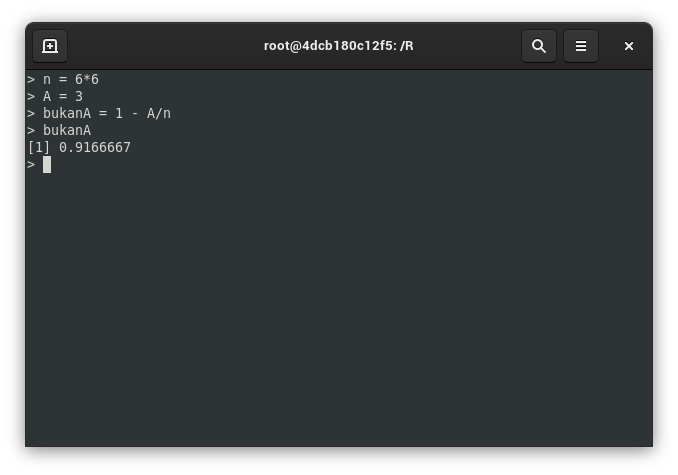
\includegraphics[scale=.5]{prak4}
\end{center}
Dua buah dadu dilambungkan bersama, maka n = 6 x 6 = 36. Jika A = {jumlah mata kedua dadu £ 3} = {(1,1), (1,2), (2,1)}. Kemudian untuk n(A) = 3, dan B = {jumlah mata kedua dadu > 3}. Bisa dilihat pada R Console dibawah, kita ketikkan n=6*6. Kemudian kita ketikkan A=3 yang artinya jumlah mata dadu sama dengan 3. Setelah itu kita ketikkan > bukanA = 1 – A/n, kemudian kita panggil > bukanA , maka peluang bahwa jumlah mata kedua dadu > 3 adalah 0,9167.

\subsubsection{Praktik 5}
Pada praktik kali ini adalah menentukan peluang muncul angka dua kali dari sebuah mata uang yang dilempar dua kali. Peristiwa ini termasuk peristiwa saling bebas, karena peristiwa yang satu tidak mempengaruhi atau dipengaruhi terjadinya peristiwa yang lainnya.
\begin{center}
	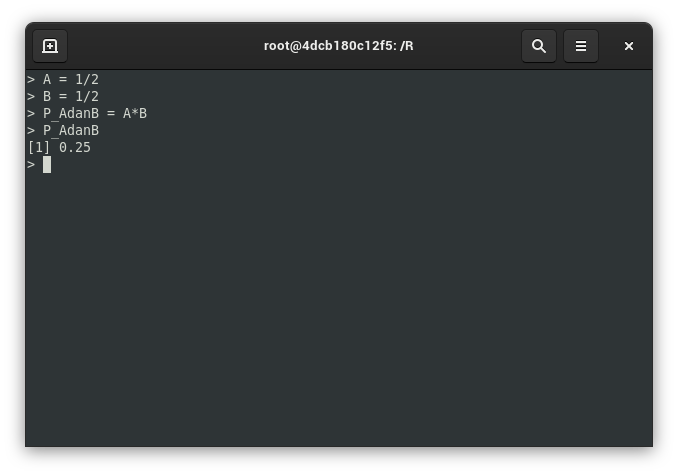
\includegraphics[scale=.5]{prak5}
\end{center}
Langkah yang dilakukan pada R Console ketikkan \\
\texttt{A=1/2 }\\
artinya dari sebuah mata uang terdapat dua kemungkinan yaitu angka atau gambar. Kemudian kita ketikkan\\ 
\texttt{B=1/2}\\ 
Setelah itu kita ketikkan\\ 
\texttt{P\_AdanB = A*B}
Kemudian kita ketikkan\\ 
\texttt{P\_AdanB} kemudian klik Enter, maka akan muncul output seperti gambar dibawah. Jadi peluang keduanya tampak angka adalah 0,25

\subsubsection{Praktik 6}
Tujuan dari praktik 6 adalah menghitung peluang kedua bola yang terambil berwarna putih, jika di dalam sebuah kotak terdapat 5 bola merah dan 4 bola putih kemudian dari dalam kotak tersebut diambil dua bola sekaligus
\begin{center}
	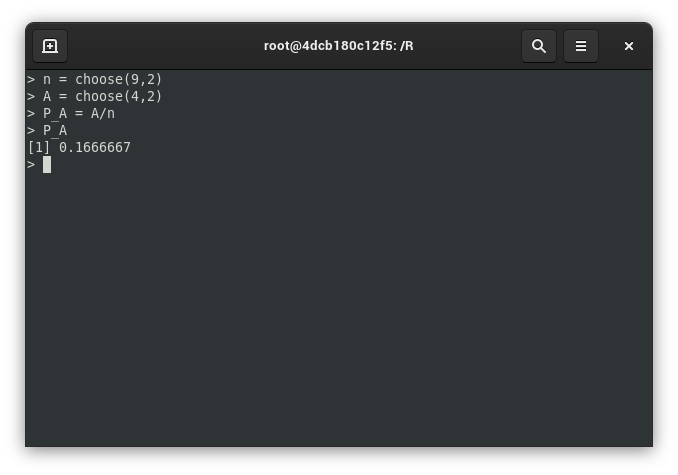
\includegraphics[scale=.5]{prak6}
\end{center}
Diketahui 
\begin{itemize}
	\item n = $_{9}C_{2}$ = 36 
	\item A = terambilnya dua bola putih 
	\item n(A) = $_{4}C_{2}$ = 6.
\end{itemize}
fungsi choose, merupakan fungsi kombinasi, maka pada R ketikkan\\
\texttt{ n = choose (9,2)}\\ 
perintah tersebut berarti n = $_{9}C_{2}$, kemudian ketikkan\\
\texttt{A = choose (4,2)}\\
kemdian kita hitung\\
\texttt{ P\_A = A/n}
kemudian panggil lagi variabel P\_A, maka peluangnya adalah 0,1667.

\subsection{Latihan}
\subsubsection{Latihan 1}
\paragraph{Masalah\\}
Tiga buah bola diambil secara acak dari sebuah kantong yang terdiri dari 8 bola merah dan 6 bola biru. Berapa peluang mendapatkan sedikitnya satu bola biru?
\paragraph{Penyelesaian\\}
\begin{center}
	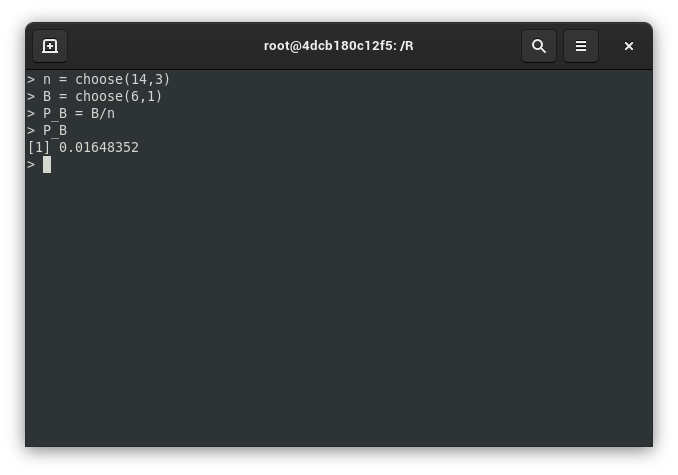
\includegraphics[scale=.5]{lat1}
\end{center}

Diketahui 
\begin{itemize}
	\item n = 14C3 = 364
	\item A = terambilnya bola biru
	\item n(A) = 6C1 = 6
	\item B = terambilnya bola merah
	\item n(B) = 8C2 = 28
\end{itemize} 
Perintah pada R Console\\ 
\texttt{n = choose (14,3)} $\rightarrow$ fungsi kombinasi dari  $_{14}C_{3}$ pada penerapannya seperti ini $_{14}C_{3} = 14!/(3!*(14-3)!)$. \\
Setelah itu kita ketikkan\\ 
\texttt{A = choose (6,1)}\\
Kemudian kita ketikkan\\ 
\texttt{B = choose (8,2)}\\ 
Selanjutnya kita beri rumus\\  
\texttt{P\_AB = A/n + B/n }, kemudian kita ketik perintah untuk memanggil variabe lagi\\ 
\texttt{P\_AB}\\ 
Maka peluang kedua bola itu berwarna putih adalah 0,0934.

\subsubsection{Latihan 2}
\paragraph{Masalah\\}
Dari setumpuk kartu bridge (52 lembar) diambil secara acak. Berapa peluang terambilnya kartu bernomor 10 atau kartu AS?
\paragraph{Penyelesaian\\}
\begin{center}
	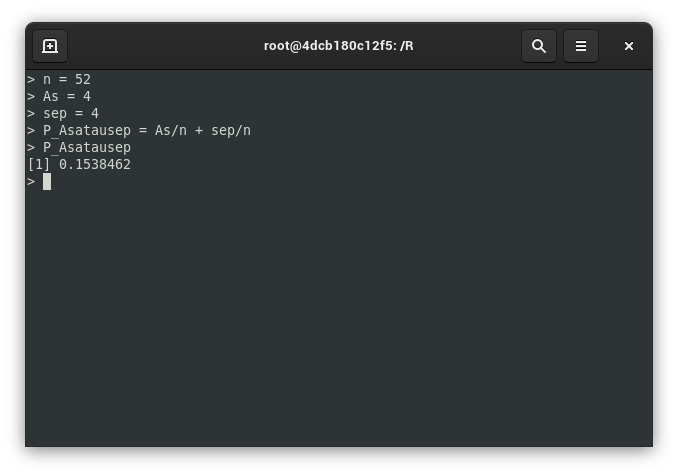
\includegraphics[scale=.5]{lat2}
\end{center}

Diketahui 
\begin{itemize}
	\item n = 52 
	\item As = 4 
	\item sep = 10
\end{itemize}. 
Pada R Console ketikkan 
\\\texttt{n = 52}
Kemudian kita ketikkan\\ 
\texttt{As = 4 } $\rightarrow$ As adalah 4 Kartu AS \\
kemudian kita ketikkan lagi\\ 
\texttt{sep = 4} $\rightarrow$ sep adalah 4 kartu bernomor 10.\\ 
Setelah itu kita ketikkan  \\
\texttt{P\_Asatausep = As/n + sep/n}.\\ 
Maka peluang terambilnya kartu AS atau kartu bernomor 10 adalah 0,1538.

\subsubsection{Latihan 3}
\paragraph{Masalah\\}
Dari satu kelas terdiri dari 35 siswa, setelah didata ternyata 20 siswa senang bermain bola basket, 18 siswa senang bermain bola volley dan 8 siswa senang keduang. Jika dipanggil salah satu siswa secara acak, maka berapa peluang yang terpilih itu senang bermain basket atau bola volley?
\paragraph{Penyelesaian\\}
\begin{center}
	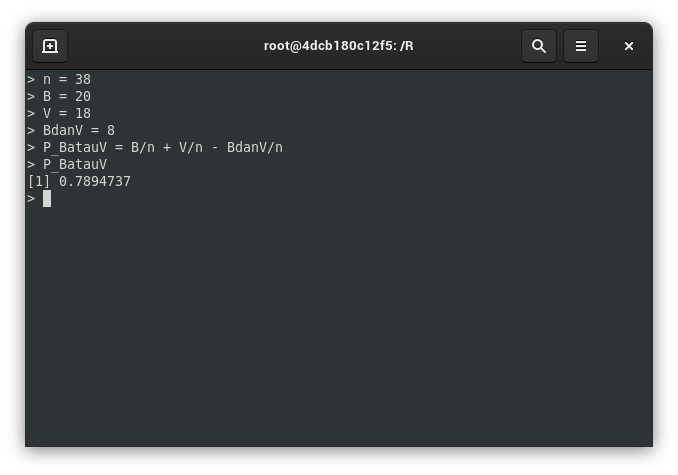
\includegraphics[scale=.5]{lat3}
\end{center}

Diketahui 
\begin{itemize}
	\item n = 35 
	\item B = 20
	\item V = 18
	\item B dan V = 8
\end{itemize}
Untuk mencari nilai peluangnya kita ketikkan\\ 
\texttt{> P\_BatauV = B/n + V/n – BdanV/n}\\ 
maka peluang yang terpilih senang bermain basket atau volley adalah 0,857

\subsubsection{Latihan 4}
\paragraph{Masalah\\}
Jika peluang hari esok akan hujan adalah 0,35, berapa peluang bahwa cuaca akan cerah esok hari?
\paragraph{Penyelesaian\\}
\begin{center}
	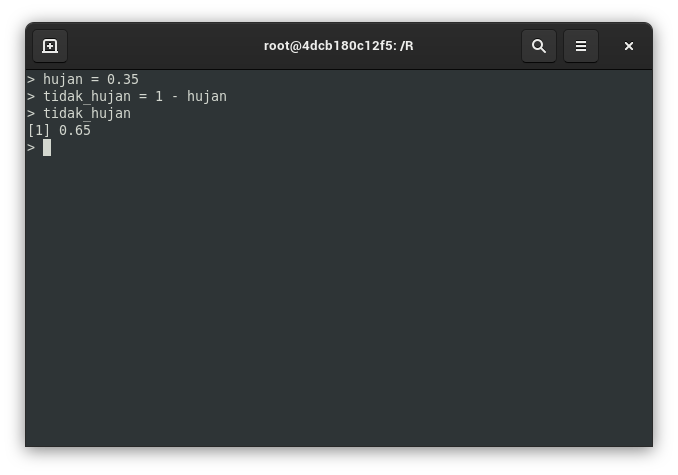
\includegraphics[scale=.5]{lat4}
\end{center}
buat variabel Hujan = 0.35 kemudian ketikkan rumusnya yaitu P\_cerah = 1 – Hujan. Kemudian kita ketikkan lagi P\_cerah. Maka peluang bahwa cuaca akan cerah esok hari adalah 0,65

\subsubsection{Latihan 5}
\paragraph{Masalah\\}
A menyatakan si Y akan hidup dalam tempo 80 tahun, B menyatakan si Z akan hidup dalam tempo juga 80 tahun. Jika diberikan P(A) = 0,65 dan P(B) = 0,52. Berapakah peluang si Y dan si Z dua-duanya akan hidup dalam tempo 80 tahun?
\paragraph{Penyelesaian\\}
\begin{center}
	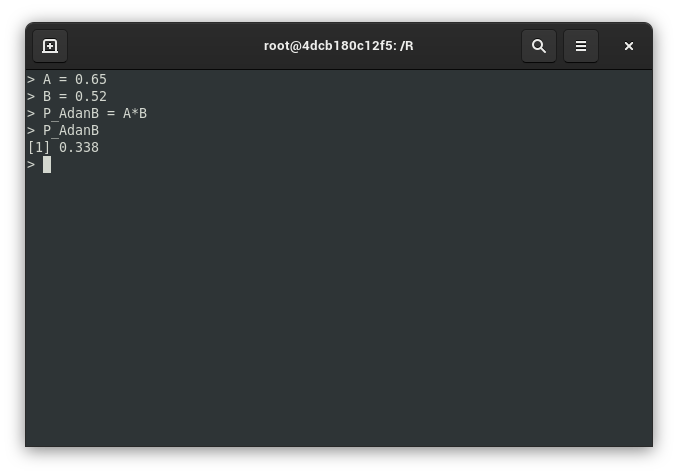
\includegraphics[scale=.5]{lat5}
\end{center}
jika A menyatakan si Y hidup dalam tempo 80 tahun, B menyatakan si Z akan hidup dalam tempo juga 80 tahun, dan diberikan P(A) = 0,65 dan P(B) = 0,52. Langkah yang dilakukan adalah pertama kita ketikkan A = 0,65, kemudian ketikkan B = 0,52. Setelah itu kita ketikkan rumusnya yaitu P\_AdanB = A*B, kemudian kita ketik P\_AdanB. Maka peluang si Y dan si Z dua-duanya akan hiidup dalam tempo 80 tahunadalah 0,338.

\subsubsection{Latihan 6}
\paragraph{Masalah\\}
Dalam sebuah kotak terdapat 30 lampu, 5 diantaranya mati (rusak). Jika diambil 5 lampu secara acak, berapa peluang mendapatkan sedikitnya 2 lampu tidak rusak?
\paragraph{Penyelesaian\\}
\begin{center}
	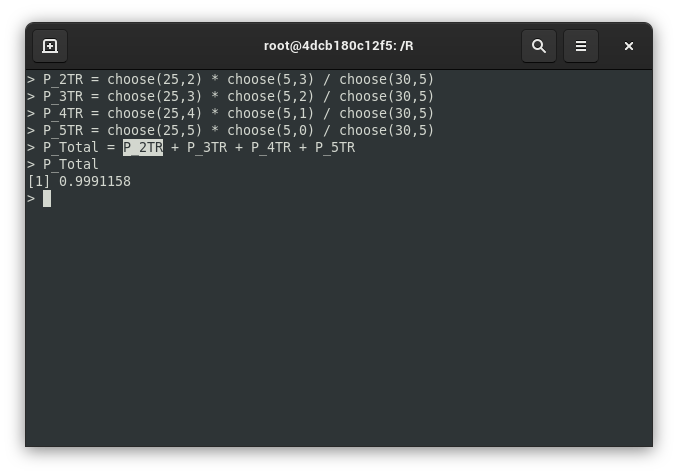
\includegraphics[scale=.5]{lat6}
\end{center}

\subsection{Tugas}
\subsubsection{Tugas 1}
\paragraph{Masalah\\}
Panitia pertunjukan panggung terbuka mengundang 10 orang penyanyi yang terdiri dari 7 wanita dan 3 pria. Berhubung keterbatasan waktu, hanya ditampilkan 5 orang penyanyi dan masing-masing penyanyi mempunyai hak yang sama untuk tampil. Berapa peluang terambilnya 5 penyanyi itu jika disyaratkan bahwa: 
\begin{enumerate}[label=\alph*.]
	\item Sekurang-kurangnya 2 penyanyi wanita.
	\item Sekurang-kurangnya 2 penyanyi pria.
\end{enumerate}

\paragraph{Penyelesaian\\}
\begin{enumerate}[label=\alph*.]
	\item 
	\begin{minipage}[t]{\linewidth}
		\raggedright
		\adjustbox{valign=t}{
			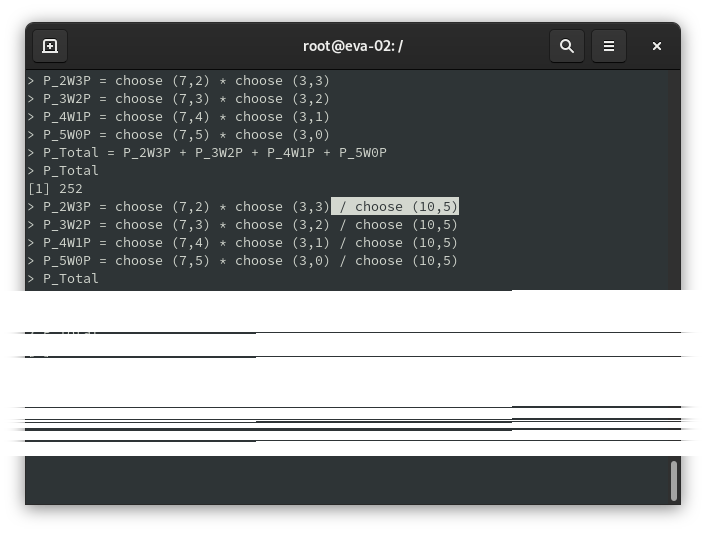
\includegraphics[width=.75\linewidth]{tugas1a}%
		}
	\end{minipage}
	\item 
	\begin{minipage}[t]{\linewidth}
		\raggedright
		\adjustbox{valign=t}{
			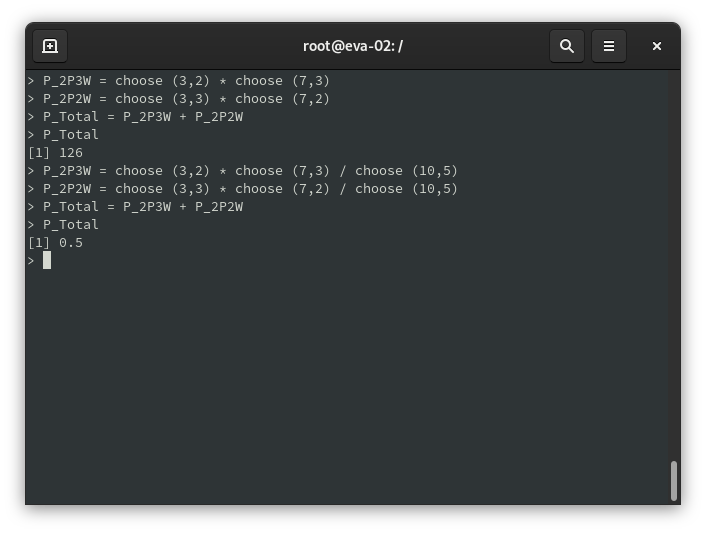
\includegraphics[width=.75\linewidth]{tugas1b}%
		}
	\end{minipage}
\end{enumerate}

\subsubsection{Tugas 2}
\paragraph{Masalah\\}
Suatu fasilitas produksi mempekerjakan 20 orang karyawannya pada shift pagi, 15 karyawan pada shift sore dan 10 orang karyawan pada shift malam. Seorang konsultan control mutu ingin memilih 6 orang karyawan untuk suatu wawancara. Misalkan pemilihan ini dilakukan sedemikian rupa sehingga kelompok 6 orang tertentu tersebut memiliki kesempatan yang sama untuk terpilih seperti hanya kelompok lainnya, tentukanlah: 
\begin{enumerate}[label=\alph*.]
	\item Probabilitas bahwa 6 karyawan yang terpilih seluruhnya berasal dari shift pagi. 
	\item Probabilitas bahwa 6 karyawan yang terpilih seluruhnya berasal dari shift yang sama. 
	\item Probabilitas bahwa 6 karyawan yang terpilih sekurang-kurangnya berasal dari dua shif yang berbeda.
\end{enumerate}

\paragraph{Penyelesaian\\}
\begin{enumerate}[label=\alph*.]
	\item 
	\begin{minipage}[t]{\linewidth}
		\raggedright
		\adjustbox{valign=t}{
			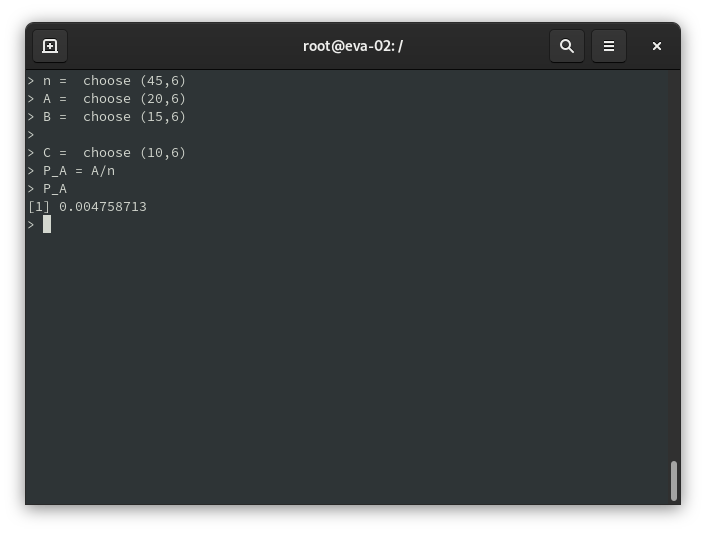
\includegraphics[width=.75\linewidth]{tugas2a}%
		}
	\end{minipage}
	\item 
\begin{minipage}[t]{\linewidth}
	\raggedright
	\adjustbox{valign=t}{
		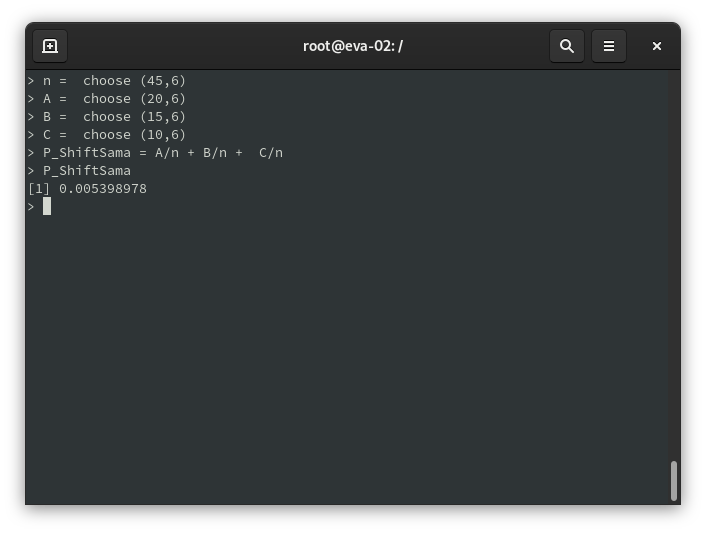
\includegraphics[width=.75\linewidth]{tugas2b}%
	}
\end{minipage}
	\item 
\begin{minipage}[t]{\linewidth}
	\raggedright
	\adjustbox{valign=t}{
		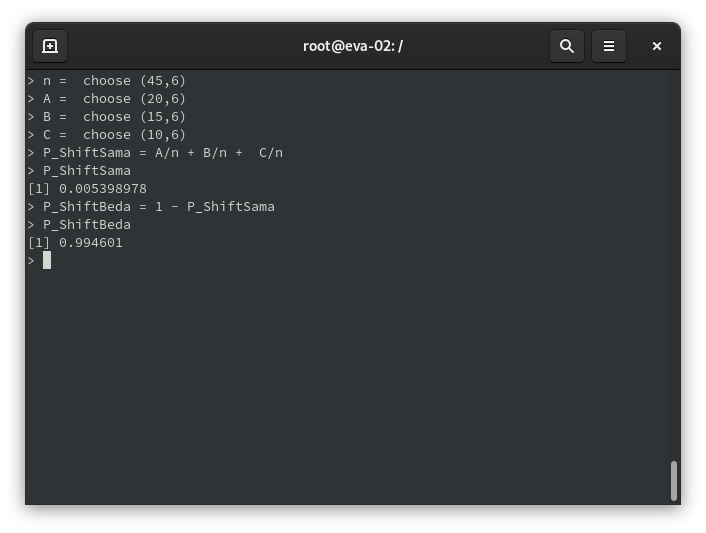
\includegraphics[width=.75\linewidth]{tugas2c}%
	}
\end{minipage}
\end{enumerate}
\newpage
\section{Kesimpulan}
Setelah saya melakukan praktikum mahasiswa lebih memahami tentang probabilitas

\end{document}